\chapter{Fundamental solutions on manifolds}
\label{chapter3}


In this chapter, the Riesz distributions will be transported on suitable domains of Lorentzian manifolds to construct local fundamental solutions and it will be discussed the local and global solvability of the Cauchy problem.\\
At first we will present some examples of generalized d'Alembert operators on some globally hyperbolic manifolds interesting for their physical applications, to show why we are interested in solving wave-like equations on manifolds and why we will follow this approach. In fact, in this setting, the methods of Fourier transform are unmanageable, but Riesz distributions are far more generalizable.\\
We will start by pulling back the Riesz distributions from the tangent space to an open neighborhood of a fixed point in a Lorentzian manifold using the exponential map and we will discuss the properties that still hold. We will see that none of the pulled back Riesz distributions defines a fundamental solution to any wave-like operator, but we can combine them in a certain way to obtain approximate fundamental solutions.\\
Precisely, we will make a formal ansatz: we will write a formal solution as a series of Riesz distributions $\mathcal{R}_\pm$ with functions as coefficients to be determined. Requiring $\mathcal{R}_\pm$ to be a fundamental solution, we will find recursive relations for the coefficients that will depend on the particular wave-like operator we are trying to solve, but that can be found in general. In this way a formal fundamental solution will be constructed as a series for which the higher terms must be cut in a precise way in order to get a true solution. We will show that it is always possible to find such a regularization $\widetilde{\mathcal{R}}_\pm$ and make the formal series converge. Unfortunately the formal series does not immediately converge to a fundamental solution, hence we will have to get rid of the difference between the true and the approximate fundamental solution, denoted by $K_\pm$, inverting the integral kernel $\mathcal{K}_\pm$ induced by $K_\pm$. We will show that this can be done only locally.\\
This considerations will lead to solutions of local Cauchy problems and we will show the regularity of such a solution with smooth initial data. Then we will generalize the results on \emph{globally hyperbolic} manifolds (see Definition \ref{defn:globalhyp}). This result will be used to show that global fundamental solutions exist in this case. All the solution will have support properties that respect the causality principle: in fact the support of any solution is contained in the union of causal future and causal past of the support of its initial data.

\section{Examples of generalized d'Alembert operators}
We recall from Section \ref{sec:operators} that a \textbf{generalized d'Alembert} operator on a manifold $\mM$ is given in local coordinates by
\begin{equation}
P=-g^{ij}(x)\frac{\partial^2}{\partial x^i\partial x^j}+a^j(x)\parz{}{x^j}+b(x),
\label{eq:generalizedAlembert}
\end{equation}
where $g^{ij}$ is the metric and $a^j$, $b$ are smooth function.\\

\noindent We now show the form of $P$, assuming for simplicity that $a^j$ and $b$ vanish, on manifolds of physical interest such as Minkowski spacetime $\mathbb{M}^n$, cosmological spacetimes or Schwartzschild spacetimes, defined in Example \ref{ex:spacetimes}.\\
In the first case, $g_{\mathbb{M}^n}=\eta$, hence the generalized d'Alembert operator coincide with the d'Alembert wave operator $\Box$.\\
For cosmological spacetimes $g_c= -\dd t^2 + f^2(t)\, b_t,$ with $f$ positive function and $b_t$ a Riemannian metric. In case $(b_t)_{ij}=\delta_{ij}\dd x_i\dd x_j$ is the euclidean metric, $g_c= -\dd t^2 + f^2(t)\sum_i\dd x_i^2$ and
\[	P_c=\frac{\partial^2}{\partial t^2}	- \frac{1}{f^2(t)}\sum_{i=1}^{n-1} \frac{\partial^2}{\partial x_i^2}.	\]
\noindent In Schwartzschild spacetime $$g_s=-h(r)\dd t^2+\frac{1}{h(r)}\dd r^2	+r^2\,g_{S^2},$$ where $h(r)=1-\frac{2m}{r}$ while $g_{S^2}=r^2\,\dd\theta^2+r^2\sin^2\theta\,\dd\varphi^2$. Hence the generalized d'Alembert operator reads
\[	P_s=	\frac{1}{h(r)}\frac{\partial^2}{\partial t^2}-{h(r)}\frac{\partial^2}{\partial r^2}-\frac{1}{r^2}\frac{\partial^2}{\partial \theta^2}-\frac{1}{r^2\sin^2\theta}\frac{\partial^2}{\partial \varphi^2}.	\]

\noindent The Fourier transform techniques rely on the translational symmetry possessed by Minkowski spacetime. Therefore, for a generic curved background, such as Schwarzschild or cosmological spacetimes, in which there is not such symmetry, the Fourier method is not well-suited. Moreover, the form assumed by the operator $P$ in the examples we covered does not posses any explicit symmetry.


\section{Local fundamental solutions}
In Section \ref{sec:riesz} Riesz distributions have been defined on the tangent spaces of an arbitrary point of a Lorentzian manifold, following [\citealp{ginoux}].
We show how to extend Riesz distributions small open subsets of the Lorentzian manifold. The step from the tangent space to the manifold will be provided by the exponential map.


\begin{definition}
	Let $\Omega\subset\mM$ be a geodesically starshaped open subset with respect to a point $x\in\mM$. For  $\alpha\in\mC$  and for every $\varphi\in\mD(\Omega\mM)$ we call Riesz distribution
	\[	\left(R_\pm^\Omega(\alpha,x),\varphi\right):=\left(R_\pm(\alpha),(\mu_x\varphi)\circ\exp_x\right),	\]
	where $\exp_x:\exp_x^{-1}(\Omega)\subset\mT_x\Omega\to\Omega$ is the exponential map at $x$ while $\mu_x:\Omega\to\mR$ is the volume form defined as in equation (\ref{eq:mu}).\\
	We call $R_+^\Omega(\alpha,x)$ and $R_-^\Omega(\alpha,x)$ respectively the \textbf{retarded} and the \textbf{advanced} Riesz distributions on $\Omega$ for $\alpha\in\mC$.
	\label{defn:rieszlocal}
\end{definition}

\noindent Note that, since $\supp\,(\mu_x\varphi)\circ\exp_x\subset\Omega$, it can be regarded as a test-function on $\mT_x\Omega$ for the Riesz distribution.\\

\noindent Distributions on a geodesically starshaped domain maintain some of the properties of the Minkowski counterpart, namely the ones expressed in Proposition \ref{prop:firstRiesz} and in Proposition \ref{prop:secondRiesz}, even if with some slight differences.

\begin{theorem}
	Let $\Omega\subset\mM$ be a geodesically starshaped open subset with respect to a point $x\in\mM$. For all $\alpha\in\mC$ it holds
	\begin{enumerate}
		\item[(1)]If $\Re\alpha>n$, then 	\begin{equation}
				R_\pm^\Omega(\alpha,x):=\begin{cases}
			C(\alpha,n)\Gamma_x^{\frac{\alpha-n}{2}}\quad &\text{on } J_{\pm}^\Omega(x)\\
			0\qquad &\text{elsewhere},\\
			\end{cases}	
		\end{equation}
		where $C(\alpha,n)$ are defined in Definition \ref{defn:Rieszmink}, while $\Gamma_x$ is defined in Definition \ref{defn:Gamma}.
		\item[(2)] $\supp\,R_\pm^\Omega(\alpha,x)\subset J_\pm(x)$.
		\item[(3)] For every $\varphi\in\mD(\Omega)$ the map $\ds\alpha\mapsto\left(R_\pm^\Omega(\alpha,x),\varphi\right)$ is holomorphic on $\mC$.
		\item[(4)] $\Gamma_x\, R_\pm^\Omega(\alpha,x)=\alpha(\alpha-n+2)R_\pm^\Omega(\alpha+2,x)$.
		\item[(5)] $\grad \Gamma_x\cdot R_\pm^\Omega(\alpha,x)=2\alpha\grad R_\pm^\Omega(\alpha+2,x)$.
		\item[(6)] $R_\pm^\Omega(0,x)=\delta_x$.
		\item[(7)] $\ds\Box R_\pm^\Omega(\alpha+2,x)=\left(\frac{\Box\Gamma_x-2n}{2\alpha}+1\right)R_\pm^\Omega(\alpha,x)$ for all $\alpha\neq0$.
		
	\end{enumerate}
\label{th:rieszdomain}
\end{theorem}
	
\noindent To prove the properties of Theorem \ref{th:rieszdomain} we need a Lemma which helps dealing with $\Gamma_x$, the function that takes the place of $\gamma$ in the formulas for the Riesz distributions on a manifold.


\begin{lem}
	Let $\Omega\subset\mM$ be an open and geodesically starshaped subset with respect to $x\in\mM$. Then it holds that
	\begin{enumerate}
		\item[(1)] $\langle\grad\Gamma_x,\grad\Gamma_x\rangle=-4\Gamma_x$;
	%	\item[(2)] On $I_+^\Omega(x)$ (respectively on$I_-^\Omega$) the vector field $\grad\Gamma_x$ is timelike \emph{past-directed} (respectively \emph{future-directed});
		\item[(2)] $\Box\Gamma_x=2n-\langle\grad\Gamma_x,\grad\ln(\mu_x)\rangle$.
	\end{enumerate}
\label{lem:rieszdomain}
\end{lem}
\Proof We prove (1) in Minkowski spacetime, where we can identify $\Gamma$ with the geodesic distance $\gamma=(x^1)^2-(x^2)^2-\cdots-(x^n)^2$. In other words
\begin{equation}
\grad\gamma=\eta^{ij}\parz{\gamma}{x^i}\parz{}{x^j}=-2x^i\parz{}{x^i}.
\label{eq:grad}
\end{equation}
Hence the first formula follows from direct computation:
\[	\begin{aligned}
\langle\grad\gamma,\grad\gamma\rangle&=\left\langle -2x^i\parz{}{x^i},-2x^i\parz{}{x^i}\right\rangle\\
&=4((x^1)^2-(x^2)^2-\cdots-(x^n)^2)\\
&=-4\gamma.
\end{aligned}	\]
To prove (2) we notice that Leibniz rule for the divergence operator reads
\begin{equation}
	\div(fZ)=f\div Z+\langle\grad f,Z\rangle,	
	\label{eq:leibdiv}
\end{equation}
for any vector field $Z$ and for any smooth function $f$ on $\mM$. Hence, equation (\ref{eq:grad}) generalizes in normal coordinates as
\[	\grad\Gamma_x=-2x^j\parz{}{x^j}.	\]
Using (\ref{eq:leibdiv}) with $f=\mu_x^{-1}$ and $Z=\grad\Gamma_x$, we obtain
\[	\div(\mu_x^{-1}\grad\Gamma_x)=\mu_x^{-1}\div\grad\Gamma_x+\langle\grad\mu_x^{-1},\grad\Gamma_x\rangle.		\]
Since
\[	\begin{aligned}
\Box\Gamma_x&=-\div\grad\Gamma_x\\
&=\mu_x\langle\grad\mu_x^{-1},\grad\Gamma_x\rangle-\mu_x\div(\mu_x^{-1}\grad\Gamma_x)\\
&=-\langle\grad\ln\mu_x,\grad\Gamma_x\rangle-\mu_x\div(\mu_x^{-1}\grad\Gamma_x),
\end{aligned}		\]
it remains to be shown that $\mu_x\div(\mu_x^{-1}\grad\Gamma_x)=-2n$.
Using the definition of divergence and equation (\ref{eq:divergence}),
\[	\mu_x\div(\mu_x\grad\Gamma_x)=\parz{}{x^j}(\grad\Gamma_x)^j=-2\parz{}{x^j}x^j=-2n.		\]
For a complete proof, we remind to [\citealp[Lem 1.3.19]{bar1}]
\endproof\\

\textbf{Proof of Theorem (\ref{th:rieszdomain}).} Let $\Re\alpha>n$, $\varphi\in\mD(\Omega)$ and let us denote with $X$ the tangent vectors in $\mT_x\Omega$. Then from Definition \ref{defn:rieszlocal},
\[ \begin{aligned}
\left(R_\pm^\Omega(\alpha,x),\varphi\right)&=\left(R_\pm(\alpha),(\mu_x\varphi)\circ\exp_x\right)\\
&=C(\alpha,n)\int_{J_\pm(0)}\gamma^{\frac{\alpha-n}{2}}(X)\mu_x\,\varphi(\exp_x(X))\,\dd X\\
&=C(\alpha,n)\int_{J_\pm^\Omega(x)}\Gamma_x^{\frac{\alpha-n}{2}}\varphi(x)\,\dd\mu.
\end{aligned}		\]
Assertions (2) and (3) follow directly from the corresponding properties of the Riesz distributions on Minkowski spacetime.\\
By (1), equation (4) holds when $\Re\alpha>n$ on account of the corresponding counterpart in the Minkowski case. By analytic extension of the distribution, it must hold in the whole complex plain.\\
To prove (5), we compute for $\Re\alpha>n$
\[	\begin{aligned}
2\alpha\grad R_\pm^\Omega(\alpha+2,x)&=2\alpha C(\alpha+2,n)\grad\Gamma_x^{\frac{\alpha+2-n}{2}}\\
&=2\alpha C(\alpha+2,n)\frac{\alpha+2-n}{2}\Gamma_x^{\frac{\alpha-n}{2}}\grad\Gamma_x\\
&=R_\pm^\Omega(\alpha,x)\grad\Gamma_x.
\end{aligned}		\]
and again we extend it for any complex $\alpha$ through analyticity.\\
To prove (6) let $\varphi\in\mD(\Omega)$. Then,
\[	\begin{aligned}
\left(R_\pm^\Omega(0,x),\varphi\right)&=\left(R_\pm(0),(\mu_x\varphi)\circ\exp_x\right)\\
&=\left(\delta_0,(\mu_x\varphi)\circ\exp_x\right)\\
&=\left((\mu_x\varphi)\circ\exp_x\right)(0)=\varphi(x)\\
&=\left(\delta_x,\varphi\right),
\end{aligned}	\]
where we used equation (2) in Proposition \ref{prop:secondRiesz}.
To prove (7) we take $\alpha\in\mC$ such that $\Re\alpha>n+2$ so that $R_\pm^\Omega(\alpha+2,x)$ is $C^2$. by the means of analytic extension of the distribution, the relation must hold for any $\alpha\in\mC$.
\[	\begin{aligned}
\Box R_\pm^\Omega(\alpha+2,x)&=-\div\grad R_\pm^\Omega(\alpha+2,x)\\
&=-\frac{1}{2\alpha}\div\left(R_\pm^\Omega(\alpha,x)\cdot\grad\Gamma_x\right)\\
&=\frac{1}{2\alpha}\Box\Gamma_x\, R_\pm^\Omega(\alpha,x)-\frac{1}{2\alpha}\langle\grad\Gamma_x,\grad R_\pm^\Omega(\alpha,x)\rangle\\
&=\frac{1}{2\alpha}\Box\Gamma_x\, R_\pm^\Omega(\alpha,x)-\frac{R_\pm^\Omega(\alpha-2,x)}{2\alpha\cdot 2(\alpha-2)}\langle\grad\Gamma_x,\grad \Gamma_x\rangle,\\
\end{aligned}		\]
and making use of equation (1) in Lemma (\ref{lem:rieszdomain}) we have
\[	\begin{aligned}
&=\frac{1}{2\alpha}\Box\Gamma_x\cdot R_\pm^\Omega(\alpha,x)+\frac{1}{\alpha(\alpha-2)}\Gamma_x R_\pm^\Omega(\alpha-2,x)\\
&=\frac{1}{2\alpha}\Box\Gamma_x\cdot R_\pm^\Omega(\alpha,x)+\frac{(\alpha-2)(\alpha-n)}{\alpha(\alpha-2)} R_\pm^\Omega(\alpha,x)\\
&=\left(\frac{\Box\Gamma_x-2n}{2\alpha}+1\right)R_\pm^\Omega(\alpha,x).
\end{aligned}		\]
\endproof\\

\subsection{Formal ansatz}
One may think, in analogy with the Minkowski scenario, that properties (2) and (6) expressed in the Theorem \ref{th:rieszdomain} make the Riesz distribution $R_\pm^\Omega(2,x)$ a good candidate to be a fundamental solution for $\Box$ at $x$. The situation is far more complicated: in fact, one can not compute $\Box R_\pm^\Omega(\alpha+2,x)$ for $\alpha=0$ unless $\Box\Gamma_x-2n$ vanishes identically, which in general is not the case.\\
It turns out that $R_\pm^\Omega(2,x)$ does not suffice to construct fundamental solutions and to this end also $R_\pm^\Omega(2k+2,x)$ for $k\geq 1$ are needed.\\

\noindent Let $\Omega$ be a geodesically starshaped open subset with respect to a given $x\in\mM$ so that the Riesz distributions are well defined. We look for fundamental solutions $\mathcal{R}_\pm$ for a generalized d'Alembert operator $P$, defined in equation \eqref{eq:generalizedAlembert}. We want to combine them in order to have a formal series, with unknown coefficients, and make it converge under suitable conditions.
We make a formal ansatz following [\citealp{ginoux}] and [\citealp[Sec 2.2.1]{bar2}]: we look for fundamental solutions for $P$ of the form

\begin{equation}
	\mathcal{R}_\pm(x)=\sum_{k=0}^{\infty} V_x^k\cdot R_\pm^\Omega(2k+2,x),
	\label{eq:formalseries}
\end{equation}
where for each $k$, $V_x^k$ is a smooth function yet to be found.\\

\noindent The series above is only formal, but applying $P$ term to term and requiring $\mathcal{R}_\pm(x)$ to be a fundamental solution one has 
\[	P\mathcal{R}_\pm(x)=\sum_{k=0}^{\infty} P\left(V_x^k\cdot R_\pm^\Omega(2k+2,x)\right)=\delta_x.	\]
Hence, one can translate the condition of $\mathcal{R}_\pm(x)$ being a fundamental solution at $x$ into conditions on the $V_x^k$.\\
To do this we need a lemma\footnote{see [\citealp[Lem 2.1.9]{bar2}]}.

\begin{lem}
	Let $P$ be a generalized d'Alembert operator as in equation \eqref{eq:generalizedAlembert} and let $f,g\in C^\infty(\Omega)$. Then it holds
	\[	P(fg)=\Box f\, g-2\partial_{\grad f}\,g+P(g)\, f.			\]
\end{lem}
Using the last lemma with $f=R_\pm^\Omega(2k+2,x)$, $g=V_x^k$ and properties (4), (5) and (7) in
Theorem \ref{th:rieszdomain} we compute
\[R_\pm^\Omega(0,x)=\sum_{k=0}^{\infty} P\left(V_x^k\cdot R_\pm^\Omega(2k+2,x)\right)=\]
\[	\begin{aligned}
&=\sum_{k=0}^{\infty} \left\{V_x^k\cdot \Box R_\pm^\Omega(2+2k,x)-2\partial_{\grad R_\pm^\Omega(2+2k,x)}V_x^k
+PV_x^k\cdot R_\pm^\Omega(2k+2,x)  \right\}\\
%&=V_x^0\cdot \Box R_\pm^\Omega(2,x)-2\partial_{\grad R_\pm^\Omega(2,x)}V_x^0+\\
%&+\sum_{k=1}^{\infty} \left\{V_x^k\cdot \left(\tfrac{\tfrac12\Box\Gamma_x-n}{2k}+1\right)R_\pm^\Omega(2k,x)-\tfrac2{4k}\partial_{\grad \Gamma_xR_\pm^\Omega(2k,x)}V_x^k+PV_x^{k-1}\cdot R_\pm^\Omega(2k,x)  \right\}\\
&=V_x^0\cdot \Box R_\pm^\Omega(2,x)-2\partial_{\grad R_\pm^\Omega(2,x)}V_x^0+\\
&+\sum_{k=1}^{\infty} \tfrac1{2k}\left\{V_x^k\left(\tfrac12\Box\Gamma_x-n+2k\right)-\partial_{\grad \Gamma_x}V_x^k+2kPV_x^{k-1}  \right\}R_\pm^\Omega(2k,x).\\
\end{aligned}		\]
Identifying the coefficients in front of $R_\pm^\Omega(2k,x)$ we get the conditions
\begin{subequations}
\begin{align}
	\text{for }&k=0\quad 2\partial_{\grad R_\pm^\Omega(2,x)}V_x^0-\Box R_\pm^\Omega(2,x)\,V_x^0+R_\pm^\Omega(0,x)=0,	\label{eq:hada1}\\
	\text{for } &k\geq 1\quad \partial_{\grad\Gamma_x}V_x^k-\left(\frac12\Box\Gamma_x-n+2k \right)V_x^k=2k\,PV_x^{k-1}.	\label{eq:hada2}
\end{align}
\end{subequations}
For consistency with the Minkowski case, between the functions that solve \eqref{eq:hada1}, one chooses $V_x^0(x)\equiv1$. To see why, one has to recall that if  $P=\Box$ in Minkowski, $R_\pm(2)$ are fundamental solutions (see Proposition \ref{prop:secondRiesz}), hence the correspondent series \eqref{eq:formalseries} has to stop at $k=0$ and the coefficient $V_x^0(x)$ has to be unitary. 


%put $k=0$ in equation \eqref{eq:hada2}. One obtains, multiplying equation \eqref{eq:hada2} by %$R_\pm^\Omega(\alpha,x)$
%\[	\partial_{\grad\Gamma_xR_\pm^\Omega(\alpha,x)}V_x^0-\left(\frac12\Box\Gamma_x-n	\right)V_x^0\,R_\pm^\Omega(\alpha,x)=0	\]
%which entails
%\[	\partial_{2\alpha\grad R_\pm^\Omega(\alpha+2,x)}V_x^0-\left(\alpha\Box R_\pm^\Omega(\alpha+2,x)-\alpha R_\pm^\Omega(\alpha,x)\right)V_x^0=0.		\]
%Dividing by $\alpha$ and taking the limit for $\alpha\to0$ we obtain
%\[	2\partial_{\grad R_\pm^\Omega(2,x)}V_x^0-\left(\Box R_\pm^\Omega(2,x)- R_\pm^\Omega(0,x)\right)V_x^0=0,		\]
%which is identical to \eqref{eq:hada1} if and only if $V_x^0(x)\equiv1$.\\

\begin{definition}
	Let $\Omega\subset\mM$ be a geodesically starshaped open subset with respect to $x\in\mM$ and $P$ a generalized d'Alembert operator as in equation \eqref{eq:generalizedAlembert}. A sequence of \textbf{Hadamard coefficients} for $P$ at $x\in\Omega$ is a sequence $\{V_x^k\}_{k\in\mathbb{N}}$ of $C^\infty(\Omega)$ which fulfills equation \eqref{eq:hada2} with $V_x^0(x)=1$ for all $x\in\Omega$.
\end{definition}

\noindent Hence, in order to construct, at least formally, fundamental solutions, the coefficients must satisfy the differential equation \eqref{eq:hada2}. These turn out to be identifiable recursively without further assumption.\\
A simple case in which an explicit formula for the coefficients can be obtained when $P$ has no first order derivatives\footnote{see [\citealp[Prop 1]{ginoux}] and [\citealp[Prop 2.2.4]{bar2}] for the general case}.\\

\noindent Let $\Phi:\Omega\times[0,1]\to\Omega$ be such that $\Phi(y,s)=\exp_x(s\cdot\exp_x^{-1}(y))$, which is well defined and smooth since $\Omega$ is a geodesically starshaped set. In other words, $\Phi$ is a parametrization of the geodesic connecting $x$ to another point $y\in\Omega$, as one can see in \textsc{Figure} \ref{fig:mapphi}.

\begin{figure}
	\centering
	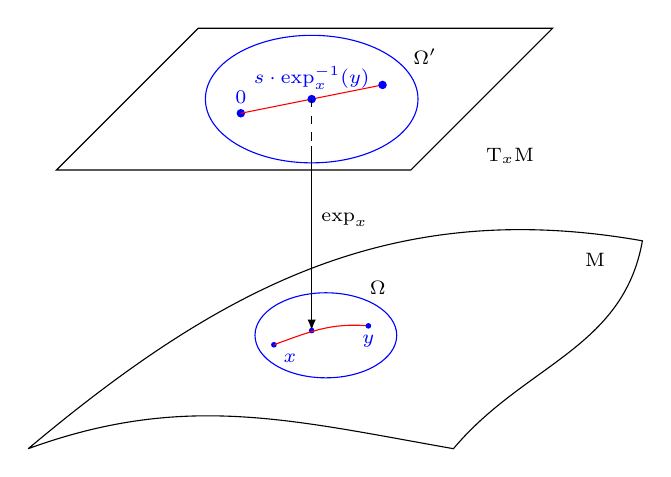
\begin{tikzpicture}[scale=1.2]
	\tikzstyle{every node}=[font=\scriptsize]
	
	\draw (1,2.8) to[out=40,in=170] (7.5,5) node at (7,4.8) {$\mathrm{M}$} to[out=-100,in=50]  (5.5,2.8) to[out=170,in=20] (1,2.8);
	
	\begin{scope}[shift={(-2,0.5)},scale=1.5]
	\node at (5.4,3.6) {$\mathrm{T}_x\mathrm{M}$};
	%\clip (2.2,3.6)-- (4.7,3.5) -- (5.7,4.5) -- (3.2,4.5) -- cycle;
	\draw [draw=black, fill=white] (2.2,3.5)-- (4.7,3.5) -- (5.7,4.5) -- (3.2,4.5) -- cycle;
	\fill [blue] (3.5,3.9) circle (0.03cm) node [above] {$0$};
	\draw [draw=blue, rotate around={0:(4,4)}] (4,4) ellipse (0.75cm and 0.45cm);
	\draw[red] (3.5,3.9) -- (4.5,4.1);
	\fill [blue] (4.5,4.1) circle (0.03cm);
	\fill [blue] (4,4) circle (0.03cm) node[above] {$s\cdot\exp_x^{-1}(y)$};
	\node at (4.8,4.3) {$\Omega'$};
	\end{scope}
	
	\begin{scope}[shift={(4,6.5)},scale=1]
	\clip (0,0) ellipse (0.75cm and 0.45cm);
	\end{scope}
	
	
	\draw [ dashed] (4,6.5) -- (4,6);
	\draw [ -latex] (4,6) -- (4,4.05) node [pos=0.4, right] {$\exp_x$};
	\fill [blue] (4,4.05) circle (0.03cm);
	\node at (4.7,4.5) {$\Omega$};
	
	\begin{scope}[shift={(0,0)},scale=1]
	%\clip (2.2,3.6)-- (4.7,3.5) -- (5.7,4.5) -- (3.2,4.5) -- cycle;
	\fill [blue] (3.6,3.9) circle (0.03cm) node [below right] {$x$};
	\draw [draw=blue, rotate around={0:(4,4)}] (4.15,4) ellipse (0.75cm and 0.45cm);
	
	\draw[red] (3.6,3.9) to[out=20,in=175] (4.6,4.1);
	
	\fill [blue] (4.6,4.1) circle (0.03cm) node [below] {$y$};
	\end{scope}
	
	\begin{scope}[shift={(4,4)},scale=1]
	\clip (0.15,0) ellipse (0.75cm and 0.45cm);
	
	\end{scope}
	
	
	\end{tikzpicture}
	\caption{The action of the map $\Phi$.}
	\label{fig:mapphi}
\end{figure}
	



\begin{theorem}
	Let $\Omega\subset\mM$ be a geodesically starshaped open subset with respect to $x\in\mM$. Let $P$ be a generalized d'Alembert operator of the form $P=\Box+\mathrm{V}$, where $\mathrm{V}\in C^\infty(\mM)$. Then there exist unique Hadamard coefficients $V_x^k$ for $P$ at $x$ given by
	\begin{equation}
		V_x^0(y)=\mu_x^{-\frac12}(y)
		\label{eq:hadamard1}
	\end{equation}	
	and for $k\geq 1$
	\begin{equation}
		V_x^k(y)=-k\mu_x^{-\frac12}(y)\int_{0}^{1}\mu_x^{\frac12}\left(\Phi(y,s)\right)s^{k-1}\,\left((PV_x^{k-1})\Phi(y,s)\right)\,\dd s.
		\label{eq:hadamard2}	
	\end{equation}		
\end{theorem}


\noindent If the point $x$ vary and if $\Omega$ is convex, the Riesz distributions are defined for all $x\in\Omega$. Write $V^k (x, y) := V_x^k (y)$ for the Hadamard coefficients at $x$, equations \eqref{eq:hadamard1} and \eqref{eq:hadamard2} imply that $V^k\in C^\infty(\Omega\times\Omega)$.

\begin{definition}
	Let $\Omega\subset\mM$ be convex and $P$ a generalized d'Alembert operator as in equation \eqref{eq:generalizedAlembert}. We call \begin{equation}
		\mathcal{R}_\pm(x)=\sum_{k=0}^{\infty} V^k(x,\cdot)\, R_\pm^\Omega(2k+2,x),
	\end{equation} the \textbf{retarded} or \textbf{advanced} formal fundamental solutions for $P$ at $x\in\Omega$.
\end{definition}
\begin{rem}
	The coefficients $V^k\in C^\infty(\Omega\times\Omega)$ can be calculated by the analogous of equations \eqref{eq:hadamard1} and \eqref{eq:hadamard2}:
	\[		V^0(x,y)=\mu_x^{-\frac12}(y),		\]
	\[		V^k(x,y)=-k\mu_x^{-\frac12}(y)\int_{0}^{1}\mu_x^{\frac12}\left(\Phi(y,s)\right)s^{k-1}\,\left((P_{(2)}V^{k-1})\Phi(y,s)\right)\,\dd s,		\]
	where the subscript $"(2)"$ in $P_{(2)}V^{k-1}$ stands for $P$ acting on the second variable, i.e. on $s\mapsto V^{k-1}(\cdot,s)$.
\end{rem}


\subsection{Approximate fundamental solutions}
The series defining $\mathcal{R}_\pm(x)$ may diverge, hence it does not provide any local fundamental solution. The idea is to make the series convergent by keeping the first terms of the formal series and multiplying the higher ones by suitable cut-off functions\footnote{see [\citealp[Lem 2.2.6]{bar2}]}.\\
Let $\Omega'$ be a convex subset. Fix an integer $N\geq \frac{n}2$. Then, for all $k\geq N$, the distribution $R_\pm^{\Omega'}(2k+2,x)$ is continuous on $\Omega'$. We split the formal fundamental solutions
\[		\mathcal{R}_\pm(x)=\sum_{k=0}^{N-1} V^k(x,\cdot)\, R_\pm^{\Omega'}(2k+2,x)	+\sum_{k=N}^{\infty} V^k(x,\cdot)\, R_\pm^{\Omega'}(2k+2,x).	\]

\begin{prop}
	Let $\Omega\subset\Omega'$ be a relatively compact open subset. Let $\sigma:\mR\to[0,1]$ be a smooth cut-off function with $\supp\,\sigma\subset[-1,1]$ and $\sigma=1$ on $[-\frac12,\frac12]$. Then there exists a sequence $\{\epsilon_k\}_{k\geq N}$ in $(0,1]$, such that, for each $j\geq 0$, the series
	\[		(x,y)\mapsto\sum_{k=N+j}^{\infty}\sigma\left(\frac{\Gamma_x(y)}{\epsilon_k}\right)V^k(x,y)R_\pm^{\Omega'}(2+2k,x)(y)=\]
	\begin{equation}
		=\begin{cases}
		\sum_{k=N+j}^{\infty} C(2+2k,n)\sigma\left(\frac{\Gamma_x(y)}{\epsilon_k}\right)V^k(x,y)\Gamma_x(y)^{k+1-\frac{n}2}\quad\text{if }&y\in J_\pm^{\Omega'}(x)\\
		0 &\text{otherwise}
		\end{cases}
	\end{equation}
	converges in $C^j(\overline{\Omega}\times\overline{\Omega})$. In particular the series
	\[	(x,y)\mapsto\sum_{k=N}^{\infty}\sigma\left(\frac{\Gamma_x(y)}{\epsilon_k}\right)V^k(x,y)R_\pm^{\Omega'}(2+2k,x)(y)		\]
	defines a continuous function.
	\label{prop:cutoff}
\end{prop}

\noindent We the main tools that we need to approximate the fundamental solutions\footnote{see [\citealp[Prop 2.2.10]{bar2}]}.


\begin{theorem}
	Let $\Omega'$ be a convex open subset of $\mM$, let $P$ be a generalized d'Alembert operator over $\mM$, as in equation \eqref{eq:generalizedAlembert}, and $\sigma$ a cut-off function per Proposition \ref{prop:cutoff}. Then, for every relatively compact open subset $\Omega\subset\Omega'$, there exists a positive sequence $\{\epsilon_k\}_{j\geq N}$, such that for every $x\in\overline{\Omega}$
	\begin{equation}
		\widetilde{\mathcal{R}}_\pm(x)=\sum_{k=0}^{N-1} V^k(x,\cdot)\, R_\pm^{\Omega'}(2k+2,x)	+\sum_{k=N}^{\infty}\sigma\left(\tfrac{\Gamma_x(y)}{\epsilon_k}\right) V^k(x,\cdot)\, R_\pm^{\Omega'}(2k+2,x)
		\label{eq:approx}
	\end{equation}
	defines a distribution on $\Omega$ satisfying
	\begin{enumerate}
		\item[(1)] $\supp\,\widetilde{\mathcal{R}}_\pm(x)\subset J_\pm^\Omega(x)$,
		\item[(2)] $P_{(2)}\widetilde{\mathcal{R}}_\pm(x)=\delta_x+K_\pm(x,\cdot)$ where $K_\pm\in C^\infty(\overline{\Omega}\times\overline{\Omega})$,
		\item[(3)] for every $\varphi\in\mD(\Omega)$, $x\mapsto\left(\widetilde{\mathcal{R}}_\pm(x),\varphi\right)$ is smooth on $\Omega$.
	\end{enumerate}
\label{th:approx}
\end{theorem}
\noindent With a suitable sequence $\{\epsilon_k\}$ the distributions defined in equation \eqref{eq:approx}, called approximate \textbf{retarded} or \textbf{advanced} fundamental solutions, approximate the true fundamental solutions, namely the difference $P_{(2)}\widetilde{\mathcal{R}}_\pm(x)-\delta_x$ is a smooth function.

\subsection{True fundamental solutions}
We can turn the approximate fundamental solution into a true one getting rid of the error terms\footnote{we will follow [\citealp[Sec 3.3.3]{ginoux}] and [\citealp[Sec 2.2.3]{bar2}]}.\\ To start with, notice that, if a sequence $\{\epsilon_k\}$ gives an approximate fundamental solution for $\Omega$, the same sequence still provides an approximate fundamental solution for any $\Omega_1\subset\Omega$.\\

\noindent We can read $K_\pm\in C^\infty(\overline{\Omega}\times\overline{\Omega})$ as an integral kernel defining the smooth integral operator for any $x\in\Omega$ and for any $u\in C^0(\Omega)$
\begin{equation}
	(\mathcal{K}_\pm u)(x):=\int_{\Omega}K_\pm(x,y)u(y)\,\dd\mu(y).
\end{equation}
Since the map $\varphi\mapsto(\delta_x,\varphi):\mD(\Omega)\to\mD(\Omega)$ is the identity operator $\id|_{\mD(\Omega)}$, one can rewrite equation (2) in Theorem \ref{th:approx} as
\[	\left(P_{(2)}	\widetilde{\mathcal{R}}_\pm(x),\varphi\right)=(\id+\mathcal{K}_\pm)\,\varphi,	\]
for all $\varphi\in\mD(\Omega)$.\\
We look for an inverse of $(\id+\mathcal{K_\pm})$. Its importance can be appreciated by observing that for all $\varphi\in\mD(\Omega)$
\begin{equation}
	(G_\pm^\Omega,\varphi):=(\id+\mathcal{K_\pm})^{-1}\left(y\mapsto\left(\widetilde{\mathcal{R}}_\pm(y),\varphi\right)\right).
	\label{eq:truelocal}
\end{equation}
Hence
\[	\begin{aligned}
\left(PG_\pm^\Omega(x),\varphi\right)&=\left(G_\pm^\Omega(x),P^*\varphi\right)\\
&=\left[	(\id+\mathcal{K_\pm})^{-1}\left(y\mapsto\left(\widetilde{\mathcal{R}}_\pm(y),P^*\varphi\right)\right)	\right](x)\\
&=\left[	(\id+\mathcal{K_\pm})^{-1}\left(\underbrace{y\mapsto\left(P_{(2)}\widetilde{\mathcal{R}}_\pm(y),\varphi\right)}_{(\id+\mathcal{K}_\pm)\,\varphi}\right)	\right](x)\\
&=\varphi(x),
\end{aligned}			\]
that is $PG_\pm^\Omega(x)=\delta_x$. If we can identify an inverse for $\id+\mathcal{K}_\pm$ and if we can prove that $G_\pm^\Omega$ is a well-defined distribution, we obtain a local \textbf{exact} fundamental solution.\\
The idea is to use the fact that, given a bounded operator $A$ on a Banach space, an operator of the form $(\id+A)$ is invertible if $\norm{A}<1$. In our case this condition can be satisfied on domains with \emph{small} volume. To be more precise we have the following proposition\footnote{see [\citealp[Lem 2.4.8]{bar1}]}:

\begin{prop}
 Let $\Omega\subset\Omega'$ be a relatively compact open and causal set (see Definition \ref{defn:pastcompact}) and assume \begin{equation}
 	|\overline{\Omega}|\,\cdot \sup_{(x,y)\in\overline{\Omega}\times\overline{\Omega}}K_\pm(x,y)<1,
 	\label{eq:small}
 \end{equation} where $|\overline{\Omega}|=\int_{\overline{\Omega}}\dd\mu$. Then $(\id+\mathcal{K}_\pm):C^k(\overline{\Omega})\to C^k(\overline{\Omega})$ is an isomorphism for all $k\in\mathds{N}$.
 \label{prop:piccolezza}
\end{prop}
\noindent The main results are:
\begin{theorem}
	Let $P$ be a generalized d'Alembert operator on $\mM$ as in equation \eqref{eq:generalizedAlembert}. Then every point of $\mM$ possesses a relatively compact causal open neighborhood $\Omega$ such that
	\begin{itemize}
	\item[(1)] 	$G_\pm^\Omega(x)$, defined in equation \eqref{eq:truelocal}, are fundamental solutions for $P$ at $x$ over $\Omega$,
	\item[(2)] $\supp\,G_\pm^\Omega(x)\subset J_\pm^\Omega(x)$, i.e. $G_\pm^\Omega(x)$ are a \textbf{retarded} and an \textbf{advanced} fundamental solution,
	\item[(3)] $\varphi\mapsto (G_\pm^\Omega(x),\varphi)$ is smooth for all $\varphi\in\mD(\Omega)$.
	\end{itemize}
\end{theorem}

\subsection{Asymptotic behaviour}

	The formal fundamental solution is asymptotic in the sense that the true fundamental solution coincides with the truncated one
	\[	\mathcal{R}_\pm	^{N+j}(x)=\sum_{k=0}^{N-1+j}V^k(x,\cdot)\, R_\pm^{\Omega'}(2+2k,x),	\]
	up to an error term which is regular on the light cone. More precisely, for all $j\in\mathbb{N}$ the map
	\begin{equation}
		(x,y)\mapsto(G_\pm^\Omega(x)-\mathcal{R}_\pm^{N+j}(x))(y)
		\label{eq:error}
	\end{equation}
	is in $C^k(\Omega\times\Omega)$. Moreover it holds:
	\begin{prop}
		For every $j\in\mathbb{N}$ there exists a constant $C_j$ such that
		\[	\sup_{(x,y)\in\overline{\Omega}\times\overline{\Omega}}(G_\pm^\Omega(x)-\mathcal{R}_\pm^{N+j}(x))(y)\leq C_j|\Gamma_x(y)|^j,			\]
		for all $(x,y)\in\Omega\times\Omega$.
		\label{prop:asymptotic}
	\end{prop}
	\noindent To prove this proposition we need a lemma\footnote{see [\citealp[Lem 2.2.20]{bar2}]}.
	
	\begin{lem}
		Let $f\in C^{3j+1}(\mathbb{M}^n)$ such that $f=0$ if $\norm{x}<0$. Then there exists a contiunuous function $h:\mathbb{M}^n\to\mR$ such that
		\[		f(x)=h(x)\gamma(x)^j,	\]
		where $\gamma(x)=-\langle x,x\rangle$.
		\label{lem:gamma}
	\end{lem}
\noindent\textbf{Proof of Proposition \ref{prop:asymptotic}.} Using the properties expressed in Theorem \ref{th:rieszdomain}, we find constants $C_k'$ such that
\[	\begin{aligned}
(&G_\pm^\Omega(x)-\mathcal{R}_\pm^{N+j}(x))(y)=\\
&=(G_\pm^\Omega(x)-\mathcal{R}_\pm^{N+3j+1}(x))(y)+\sum_{k=N+j}^{N+3j}V^k(x,y)\,R_\pm^{\Omega'}(2+2k,x)(y)\\
&=(G_\pm^\Omega(x)-\mathcal{R}_\pm^{N+3j+1}(x))(y)+\\
&+\sum_{k=N+j}^{N+3j}V^k(x,y)\,C_k'\,\Gamma_x(y)^j\,R_\pm^{\Omega'}(2+2(k-j),x)(y).
\end{aligned}		\]
The function $h_k(x,y):=C_k'\,V^k(x,y)\,R_\pm^{\Omega'}(2+2(k-j),x)(y)$ is continuous since $2+2(k-j)\geq 2+2N\geq2+n>n$. In view of equation \eqref{eq:error}, the function $(x,y)\mapsto(G_\pm^\Omega(x)-\mathcal{R}_\pm^{N+3j+1}(x))(y)$ is $C^{3j+1}$ and $\supp\,(G_\pm^\Omega(x)-\mathcal{R}_\pm^{N+3j+1}(x))\subset J_\pm^\Omega(x)$. We apply Lemma \ref{lem:gamma} in normal coordinates (note that $\Gamma_x(y)=\gamma(\exp_x^{-1}(y))$) and find a continuous function $h$ such that
\[	(G_\pm^\Omega(x)-\mathcal{R}_\pm^{N+3j+1}(x))(y)=h(x,y)\,\Gamma_x(y)^k.			\]
Hence,
\[	(G_\pm^\Omega(x)-\mathcal{R}_\pm^{N+j}(x))(y)=\left(h(x,y)+\sum_{k=N+j}^{N+3j}h_k(x,y)\right)\,\Gamma_x(y)^j.		\]
If we now set $C_j:=\sup_{(x,y)\in\overline{\Omega}\times\overline{\Omega}}\left(h(x,y)+\sum_{k=N+j}^{N+3j}h_k(x,y)\right)$ the proposition is proven.\endproof\\


\subsection{Uniqueness and regularity}
We want to solve the inhomogeneous equation $Pu = \psi$ for a given $\psi$ with small support, \emph{small} in the sense of Proposition \ref{prop:piccolezza}. The support $\Omega$ is relatively compact and equation \eqref{eq:small} holds.
\begin{prop}
	Under the assumption of Proposition \ref{prop:piccolezza}, for every $\psi\in\mD(\Omega)$ there exists a function $u_\pm\in C^\infty(\Omega)$ such that
	\[	\begin{aligned}
		&Pu_\pm=\psi\\
		&\supp\,u_\pm\subset J_\pm^\Omega(\supp\,\psi).
	\end{aligned}		\]
	\label{prop:localsol}
\end{prop}
\Proof Let \begin{equation}
	(u_\pm,\varphi):=\int_{\Omega}(G_\pm^\Omega(x),\varphi)\,\psi(x)\,\dd \mu.
	\label{eq:localsol}
\end{equation}
We will not prove that equation \eqref{eq:localsol} defines a smooth function, rather only $Pu_\pm=\psi$. Let $\varphi\in\mD(\Omega)$. It holds
\[\begin{aligned}
(Pu_\pm,\varphi)&=(u_\pm,P^*\varphi)\\
&=\int_{\Omega}(G_\pm^\Omega(x),P^*\varphi)\,\psi(x)\,\dd \mu\\
&=\int_{\Omega}(\underbrace{P_{(2)}G_\pm^\Omega(x)}_{=\delta_x},\varphi)\,\psi(x)\,\dd \mu\\
&=\int_{\Omega}\varphi(x)\,\psi(x)\,\dd\mu=(\psi,\varphi).
\end{aligned}				\]
To prove the support condition, let $\varphi\in\mD(\Omega)$ such that $(u_\pm,\varphi)\neq 0$, then there exists $x\in\Omega$ such that $(G_\pm^\Omega(x),\varphi)\,\psi(x)\neq 0$, which implies $\supp\,\varphi\cap\supp\,G_\pm^\Omega(x)\neq \emptyset$ and $x\in\supp\,\psi$. Hence $\supp\,\varphi\cap J_\pm^\Omega(x)\neq\emptyset$, i.e. $x\in J_\mp^\Omega(\supp\,\varphi)$, so that $J_\mp^\Omega(\supp\,\varphi)\cap\supp\,\psi$, which is equivalent to the thesis.\endproof\\

\noindent As we mentioned in Proposition \ref{prop:paradoxes}, the topological and geometrical properties of the Lorentzian manifold may be problematic when we are looking for solutions of a differential equation. For example, even if the manifold is not compact, the existence of closed timelike loops can make the problem ill-posed.\\
To avoid these situations and to implement the causality conditions we restrict the discussion to the \textbf{globally hyperbolic} setting (see Definition \ref{defn:globalhyp}), although some results may be extended to other cases.\\

\noindent In such case the main results are

\begin{theorem}
	Let $P$ be a generalized d'Alembert operator on a globally hyperbolic spacetime $\mM$ as in equation \eqref{eq:generalizedAlembert}. Then every solution of the equation $PF=0$ in $\mD'(\mM)$ with past- or future-compact support (see Definition \ref{defn:pastcompact}) vanishes.
	\label{th:vanishes}
	
\end{theorem}
\Proofsketch Take the case $F\in\mD'(\Omega)$ with past-compact support. The thesis is $(F,\varphi)=0$ for any $\varphi\in\mD(\mM)$. The idea is to solve the inhomogeneous equation
	\[	\begin{aligned}
&P^*u=\varphi\\
&\supp\,u\subset J_-^\Omega(\supp\,\varphi)
\end{aligned}		\]
(using Proposition \ref{prop:localsol}) for any $\varphi$ such that $\supp\,\varphi$ is small in the sense expressed in Proposition \ref{prop:piccolezza}. If one proves that $\supp\, F\cap J_-^\Omega(\supp\,\varphi)$ is compact, it holds
\[	(F,\varphi)=(F,P^*u)=(PF,u)=0.		\]
The proof of such properties involves the global hyperbolicity of the manifold. For the complete proof see [\citealp[Sec 2.3]{bar2}]\endproof\\

\noindent Now uniqueness is straightforward:
\begin{cor}
	Let $P$ be a generalized d'Alembert operator on a globally hyperbolic spacetime $\mM$ as in equation \eqref{eq:generalizedAlembert} and let $x\in\mM$. Then there exist at most one retarded and at most one advanced fundamental solution for $P$ at $x$.
	\label{cor:uniquenessfundamental}
\end{cor}
\Proof Let $G_1$ and $G_2$ be two retarded fundamental solutions at $x$. Then $G = G_1-G_2$ is a solution for $PG = 0$. Since $G_1$ and $G_2$ are retarded solutions we know that $\supp\, G\subset \supp\,G_1 \cup \supp\,G_2 \subset J_+^\mM (x)$. On a globally hyperbolic manifold $J_+^\mM (x)$ is past compact. Then for Theorem \ref{th:vanishes} $G=0$ and hence $G_1=G_2$.\endproof

\section{Local and global Cauchy problem}
\label{sec:globalCauchy}
We now explore the solvability of the Cauchy problem, in analogy with Section \ref{sec:cauchymink}, in order to obtain results needed to prove the existence and uniqueness of the fundamental solutions.

\subsection{Local solvability}


Next we prove existence and uniqueness of solutions to the Cauchy problem on small domains. To start with, it is useful to show a formula that helps controlling a solution of the problem in terms of its initial data\footnote{see [\citealp[Lem 3.2.2]{bar2}]}. This theorem and its corollary are the analogous of Theorem \ref{th:deltaprimo} and Corollary \ref{cor:homogeneousmink}, which can be regarded as particular cases.

\begin{theorem}
	Let $P$ be a generalized d'Alembert operator on $\mM$, as in equation \eqref{eq:generalizedAlembert}, and let $S$ be a smooth spacelike hypersurface of $\mM$ with a timelike oriented unit normal vector field $n:S\to\mT\mM$.\\
	Let $\Omega\subset\mM$ be a \emph{small} subset in the sense of Proposition \ref{prop:piccolezza} such that $S\cap\Omega$ is a Cauchy hypersurface of $\Omega$. If $u_\pm\in C^\infty(\Omega)$
	such that $\supp\,u_\pm\subset J_\pm^\Omega(K)$ (where $K:=\supp\, u_0\cup\supp\,u_1\cup\supp\,\psi$)
	solve the Cauchy problem
	\begin{equation}
	\begin{cases}
	P u_\pm=\psi\\
	\\
	u_\pm|_{S\cap\Omega}=u_0\\
	\\
	\partial_n u_\pm|_{S\cap\Omega}=u_1,
	\end{cases}
	\end{equation}
	with $(\psi,u_0,u_1)\in\mD(\Omega)\oplus\mD(S\cap\Omega)\oplus\mD(S\cap\Omega)$, then it holds
\begin{equation}
	\begin{aligned}
	\int_{\Omega}u_\pm(x)\varphi(x)\,\dd\mu&=\int_{\Omega}\left(G_\pm^\Omega(x),\varphi\right)\psi(x)\,\dd\mu+\\
	&+\int_{S\cap\Omega}\left(\partial_n(G_\pm^\Omega(x),\varphi)u_0-(G_\pm^\Omega(x),\varphi)u_1\right)\,\dd \mu_S,
	\end{aligned}
	\label{eq:formulagenerale}
\end{equation}
	
	\noindent for all $\varphi\in\mD(\Omega)$, where $\dd \mu_S$ is the $n-1$ dimensional pull-back measure on $S$.\footnote{Pull-back measure are defined in [\citealp[Ch. 1]{pullback}]}
	\label{th:integraledisuperficie}
\end{theorem}
\begin{cor}
	In the conditions of last lemma, if $u\in C^\infty(\Omega)$ solves $Pu=0$ then
	\[\supp\,u\subset J_+^\Omega(K)\cup J_-^\Omega(K),\]
	where $K:=\supp\,u_0\cup\supp\,u_1$, and
	\begin{equation}
	\int_\Omega u(x)\varphi(x)\,\dd\mu=\int_{S\cap\Omega}\left(\partial_n(G^\Omega(x),\varphi)u_0-(G^\Omega(x),\varphi)u_1\right)\,\dd \mu_S,
	\label{eq:integraledisuperficie}
	\end{equation}
	for all $\varphi\in\mD(\Omega)$, where $G^\Omega(x)=G_+^\Omega(x)-G_-^\Omega(x)$ and where $\dd \mu_S$ is the $n-1$ dimensional pull-back measure on $S$.
	\label{cor:integraledisuperficie}
\end{cor}
\Proof We apply Theorem \ref{th:integraledisuperficie} with $\psi=0$, noting that one can write $u$ in the form $u=u_+-u_-$ such that  $\supp\,u_\pm\subset J_\pm^\Omega(K)$. Using equations \eqref{eq:formulagenerale} for both $u_+$ and $u_-$ and subtracting the outcomes, we obtain the thesis. Since $\supp\,G_\pm^\Omega(x)\subset J_\pm^\Omega(x)$, the right hand side of equation \eqref{eq:formulagenerale} vanishes outside $J_+(K)\cup J_-(K)$, hence $\supp\,u\subset J_+(K)\cup J_-(K)$.\endproof\\

\begin{theorem}
	Under the hypotheses of Lemma \ref{th:integraledisuperficie}, for each \emph{small} open subset $\Omega\subset\mM$, such that the hypotheses of Proposition \ref{prop:piccolezza} are satisfied, such that $S\cap\Omega$ is a Cauchy hypersurface of $\Omega$, it holds that for all triples $(\psi,u_0,u_1)\in\mD(\Omega)\oplus\mD(S\cap\Omega)\oplus\mD(S\cap\Omega)$ there exists a unique $u\in C^\infty(\Omega)$ with
	\begin{equation}
	\begin{cases}
	P u=\psi\\
	\\
	u|_{S\cap\Omega}=u_0\\
	\\
	\partial_n u|_{S\cap\Omega}=u_1.
	\end{cases}
	\end{equation}
	Moreover $\supp\,u\subset J_+^\Omega(K)\cup J_-^\Omega(K)$, where $K:=\supp\, u_0\cup\supp\,u_1\cup\supp\,\psi$.
	
	\label{th:localsolvability}
\end{theorem}
\Proofsketch Since causal domains are globally hyperbolic we may apply Theorem \ref{th:Bernal} to find an isometry $\Omega = \mR \times (S \cap \Omega)$, setting the metric in the form $g=-\beta\,\dd t^2+b_t$. Now we look for a formal solution
\begin{equation}
	u(t,x)=\sum_{j=0}^{\infty}t^j\,\widetilde{u}_j(x),
	\label{eq:seriesrec}
\end{equation}			
where $(t,x)\in\mR \times (S \cap \Omega)$. On $S\cap\Omega$ we set $\widetilde{u}_0=u_0$ and $\widetilde{u}_1=-(\beta)^\frac12 u_1$. The generalized d'Alembert operator can be written in the form $P=\frac1{\beta}\frac{\partial^2}{\partial t^2}+Y$, where $Y$ contains at most derivatives of order $1$ in $t$.\\
From the equation
\begin{equation}
	\psi=Pu=\left(\frac1{\beta}\frac{\partial^2}{\partial t^2}+Y\right)u=\frac1{\beta}\sum_{j=2}^{\infty}j(j-1)t^{j-2}\widetilde{u}_j	+Yu,
	\label{eq:recursive}
\end{equation}		
for $t=0$ we have
\[	2\beta(0,x)\,\widetilde{u}_2(x)=-Y(\widetilde{u}_0+t\widetilde{u}_1)(0,x)+\psi(0,x).		\]
This relation determines uniquely $\widetilde{u}_2$ from $\widetilde{u}_0$,$\widetilde{u}_1$ and $\psi|_S$. One can hence find recursive relations for $\widetilde{u}_j$ differentiating equation \eqref{eq:recursive} with respect to $t$ and repeating the procedure.\\
In general the series in equation \eqref{eq:seriesrec} is non-convergent, but one can find a suitable positive sequence $\{\epsilon_j\}$ such that the series
\[	\widehat{u}:=\sum_{j=0}^{\infty}\sigma\left(\frac{t}{\epsilon_j}\right)t^j\widetilde{u}_j,		\]
 defines a smooth function on $\Omega$ and such that $P\widehat{u}-\psi$ vanishes at least on $S\cap\Omega$. Here $\sigma$ is a cut-off function as in Proposition \ref{prop:cutoff}. Proposition \ref{prop:localsol} provides smooth solutions $\widetilde{u}_\pm$ of the inhomogeneous problems
	\[	\begin{aligned}
&P\widetilde{u}_\pm=h_\pm\\
&\supp\,\widetilde{u}_\pm\subset J_\pm^\Omega(\supp\,h_\pm),
\end{aligned}		\]
where $h_\pm|_{J_\pm^\Omega(S\cap\Omega)}:=P\widehat{u}-\psi$ vanishes everywhere else on $\Omega$. One needs to show that $u_\pm:=\widehat{u}-\widetilde{u}_\pm$ solves the equation $Pu_\pm=\psi$ on $J_\pm^\Omega(S\cap\Omega)$ and that it vanishes on $J_\mp^\Omega(S\cap\Omega)$. Then the function
\[	u:=\begin{cases}
u_+\quad\text{on }& J_+^\Omega(S\cap\Omega)\\
u_-\quad\text{on }& J_-^\Omega(S\cap\Omega)
\end{cases}		\]
is smooth and it solves the Cauchy problem.\\
Uniqueness follows from Corollary \ref{cor:integraledisuperficie}. In fact, if $u_1$ and $u_2$ solve the Cauchy problem, for linearity $u_1-u_2$ solves the problem with vanishing initial data $(\psi,u_0,u_1)\equiv(0,0,0)$. Hence $u:=u_1-u_2=0$ because of equation \eqref{eq:integraledisuperficie}. The assertion of the support follows from the corresponding one from the homogeneous problem and from Corollary \ref{cor:integraledisuperficie}. For a complete proof, see [\citealp[Prop 2.4.1]{bar2}]. \endproof\\

\begin{figure}
	\centering
	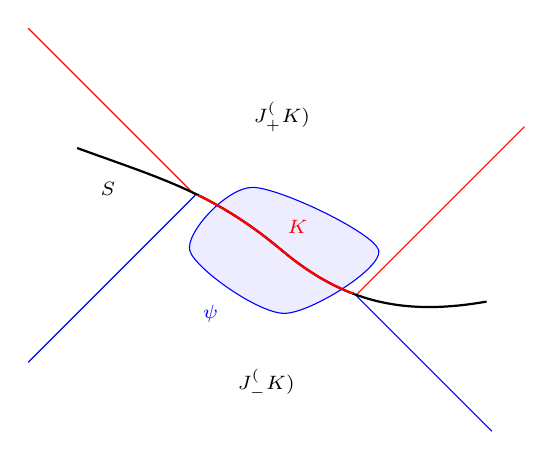
\begin{tikzpicture}
	\tikzstyle{every node}=[font=\scriptsize]
	\begin{scope}[shift={(0.33,0)},scale=0.8]
	\draw [color=blue, fill=blue, fill opacity=0.07] plot [smooth cycle] coordinates { (0,0) (1,1) (3,0) (1.5,-1)};
	
	
	\node at (0.3,-1) {\textcolor{blue}{$\supp\,\psi$}};
	\end{scope}
	
	
	
	\node at (1.7,0.3) {\textcolor{red}{$K$}};
	\begin{scope}[shift={(2.46,-0.55)},scale=1]
	\draw [color=red] (0,0) -- (45:3cm);
	\end{scope}
	
	\begin{scope}[shift={(2.4,-0.53)},scale=1]
	\draw [color=blue] (0,0) -- (-45:2.5cm);
	\end{scope}
	
	\begin{scope}[shift={(0.4,0.7)},scale=1]
	\draw [color=red] (0,0) -- (135:3cm);
	\end{scope}
	
	
	\begin{scope}[shift={(0.4,0.7)},scale=1]
	\draw [color=blue] (0,0) -- (-135:3cm);
	\end{scope}
	
	\node at (1.5,1.7) {$J_+^\mM(K)$};
	\node at (1.3,-1.7) {$J_-^\mM(K)$};
	
	\begin{scope}[shift={(1.5,0)},scale=1.3]
	\draw[thick] (-2,1) to[out=-20,in=140] (0,0) to[out=-40,in=190] (2,-0.5);
	%\draw (0,0) -- (1.1,1.1);
	%\draw (0,0) -- (-1.1,1.1);
	%\draw (0,1.1) ellipse (1.1 and 0.18);
	%\draw[fill=black] (0,0) circle (0.03cm);
	\node at (-1.7,0.6) {$S$};
	\end{scope}
	\begin{scope}
	\clip (0.4,0.7) -- (2.46,0.7) -- (2.46,-0.55) -- (0.4,-0.55) -- cycle;
	\begin{scope}[shift={(1.5,0)},scale=1.3]
	\draw[thick, red] (-2,1) to[out=-20,in=140] (0,0) to[out=-40,in=190] (2,-0.5);
	\end{scope}
	
	\end{scope}
	
	
	\end{tikzpicture}
	\caption{The support properties of the solution to the Cauchy problem. Here $K:=\supp\, u_0\cup\supp\,u_1\cup\supp\,\psi$.}
\end{figure}





\subsection{Global solvability}

The main result of this section generalizes what we obtained in Theorem \ref{th:localsolvability} to the globally hyperbolic case.

\begin{theorem}
	Let $P$ be a generalized d'Alembert operator on a globally hyperbolic spacetime $\mM$, as in equation \eqref{eq:generalizedAlembert}, and let $S$ be a smooth Cauchy hypersurface of $\mM$ with a timelike oriented unit normal vector field $n:S\to\mT\mM$.\\
	Then it holds that for all triples $(\psi,u_0,u_1)\in\mD(\mM)\oplus\mD(S)\oplus\mD(S)$ there exists a unique $u\in C^\infty(\mM)$ such that
	\begin{equation}
	\begin{cases}
	P u=\psi\\
	\\
	u|_S=u_0\\
	\\
	\partial_n u|_S=u_1.
	\end{cases}
	\end{equation}
	Furthermore $\supp\,u\subset J_+^\mM(K)\cup J_-^\mM(K)$, where $K:=\supp\, u_0\cup\supp\,u_1\cup\supp\,\psi$ and the map
	\begin{equation*}
	\begin{aligned}
	\mD(\mM)\oplus\mD(S)\oplus\mD(S)&\to C^{\infty}(\mM)\\
	(\psi,u_0,u_1)&\mapsto u.
	\end{aligned}
	\end{equation*}
	is \textbf{linear continuous}.
\end{theorem}
\Proofsketch The existence of $u$ is proved in two steps. One constructs a solution $u$ in the strip $(-\epsilon,\epsilon)\times S$ for some $\epsilon>0$ by gluing together local solutions obtained in Theorem \ref{th:localsolvability}, noting that there is only a finite number of them since the supports are compact. Then one extends $u$ in the whole future and past of the strip. For uniqueness, an argument similar to that of Theorem \ref{th:localsolvability}, which made use of Corollary \ref{cor:integraledisuperficie}, can be used.\\
The continuous dependence on the initial data can be proven with methods of functional analysis. The complete proof can be found at [\citealp[Th. 3.2.9]{bar2}]\endproof\\

\begin{rem}
	The former result can be extended further. In fact the same thesis holds even if the triple of initial data $(\psi,u_0,u_1)$ is in $C^\infty(\mM)\oplus C^\infty(S)\oplus C^\infty(S)$\footnote{see [\citealp[Cor 5]{ginoux}]}.
\end{rem}



\section{Global fundamental solutions}
Since uniqueness of the retarded and advanced fundamental solutions has already been proven in Corollary \ref{cor:uniquenessfundamental}, it remains to show the global existence.\\
We summarize the results in the following theorem\footnote{see [\citealp[Th. 4]{ginoux}]}.
\begin{theorem}
	Let $P$ be a generalized d'Alembert operator on a globally hyperbolic spacetime $\mM$, as in equation \eqref{eq:generalizedAlembert}. Then for each $x\in\mM$ there exists a unique fundamental solution $G_+(x)$ with past-compact support and a unique one $G_-(x)$ with future-compact support.\\
	Furthermore, they satisfy
	\begin{itemize}
		\item $\supp\, G_\pm\subset J_\pm^\mM(x)$,
		\item the maps $x\mapsto(G_\pm(x),\varphi)$ identify smooth functions on $\mM$ satisfying $P^*(G_\pm(\cdot),\varphi)=\varphi$, for every $\varphi\in\mD(\mM)$.
	\end{itemize}
\end{theorem}

\begin{rem}
	From the last theorem one can prove that on a globally hyperbolic spacetime, the wave-like equation $Pu=\psi$, with $\psi\in\mD(\mM)$ possesses a unique solution $u_\pm$ with $\supp\, u_+$ (respectively $\supp\, u_-$) being past (respectively future) compact.
\end{rem}

\section{Green's operators}

We want to show the strict correspondence between fundamental solutions on manifolds and the so-called \textbf{Green's operators}. They are operators which can be seen as inverses of P when restricted to suitable spaces of functions.\\

\begin{definition}
	Let $P$ be a generalized d'Alembert operator on a spacetime $\mM$. A retarded \textbf{Green's operator} for $P$ on $\mM$ is a linear map
	\[	\mathds{G}_+:\mD(\mM)\to C^\infty(\mM)		\]
	such that satisfies
	\begin{enumerate}
		\item[(1)]	$P\circ \mathds{G}_+=\id_{\mD(\mM)}$,
		\item[(2)] $\mathds{G}_+\circ P|_{\mD(\mM)}=\id_{\mD(\mM)}$,
		\item $\supp\,\mathds{G}_+\varphi\subset J_+^\mM(\supp\,\varphi)$ for all $\varphi\in\mD(\mM)$.
	\end{enumerate}
	An advanced \textbf{Green's operator} $\mathds{G}_-:\mD(\mM)\to C^\infty(\mM)$ satisfies $(1)$ and $(2)$ and $\supp\,\mathds{G}_-\varphi\subset J_-^\mM(\supp\,\varphi)$ for all $\varphi\in\mD(\mM)$.
	\label{defn:green}
\end{definition}

\noindent Next proposition shows that in fact Green's operators and fundamental solutions are two different versions of mainly the same concept.




\begin{prop}
	In the frame of the above definition, retarded (resp. advanced) Green's operators for $P$ stand in one-to-one correspondence with advanced (resp.retarded) fundamental solutions for $P^*$. More precisely, if $G_\pm(x)$ is a family of retarded or advanced fundamental solutions for the adjoint operator $P^*$ and if 
	\begin{itemize}
		\item $x\mapsto(G_\pm(x),\varphi)$ is smooth for each test-function $\varphi$,
		\item $G_\pm(x)$ satisfies the differential equation $P(G_\pm(\cdot),\varphi) = \varphi$
	\end{itemize}, then 
	\begin{equation}
	(\mathds{G}_\pm\varphi)(x):=(G_\mp(x),\varphi),
	\label{eq:green}
	\end{equation}
	defines retarded or advanced Green's operators for $P$ respectively.\\ Conversely, for every Green's operators $\mathds{G}_\pm$ for $P$, equation \eqref{eq:green} defines fundamental solutions $G_\mp(x)$ such that $x\mapsto(G_\pm(x),\varphi)$ is smooth for each test-function $\varphi$ and satisfies the differential equation $P(G_\pm(\cdot),\varphi) = \varphi$.
\end{prop}









